%\documentclass[11pt,a4paper]{report}


% The Beamer class comes with a number of default slide themes
% which change the colors and layouts of slides. Below this is a list
% of all the themes, uncomment each in turn to see what they look like.

%\usetheme{default}
%\usetheme{AnnArbor}
%\usetheme{Antibes}
%\usetheme{Bergen}
%\usetheme{Berkeley}
%\usetheme{Berlin}
%\usetheme{Boadilla}
%\usetheme{CambridgeUS}
%\usetheme{Copenhagen}
%\usetheme{Darmstadt}
%\usetheme{Dresden}
%\usetheme{Frankfurt}
%\usetheme{Goettingen}
%\usetheme{Hannover}
%\usetheme{Ilmenau}
%\usetheme{JuanLesPins}
%\usetheme{Luebeck}
%\usetheme{Madrid}
%\usetheme{Malmoe}
%\usetheme{Marburg}
%\usetheme{Montpellier}
%\usetheme{PaloAlto}
%\usetheme{Pittsburgh}
%\usetheme{Rochester}
%\usetheme{Singapore}
%\usetheme{Szeged}
%\usetheme{Warsaw}

\documentclass[10pt]{beamer}
\usepackage{float}
\usepackage[nodisplayskipstretch]{setspace}
\usepackage{pdfpages}
\usepackage{tikz}    
\usetheme{metropolis}
\usepackage{appendixnumberbeamer}
\usepackage[normalem]{ulem}
\usepackage{eurosym}
\usepackage{booktabs}
\usepackage[scale=2]{ccicons}
\usepackage[utf8]{inputenc}
\usepackage{soul}
\usepackage{mathabx}
\usepackage{graphicx}
\usepackage{pgfplots}
\usepgfplotslibrary{dateplot}
 \usepackage{relsize}
\usepackage{xspace}
\usepackage{caption}

\usepackage{graphicx}
\usepackage{graphicx}

\usepackage{hyperref}
\hypersetup{
    colorlinks=true,
    linkcolor=blue,
    filecolor=magenta,      
    urlcolor=blue,
}
 
\urlstyle{same}
\newcommand{\themename}{\textbf{\textsc{metropolis}}\xspace}


% As well as themes, the Beamer class has a number of color themes
% for any slide theme. Uncomment each of these in turn to see how it
% changes the colors of your current slide theme.

%\usecolortheme{albatross}
%\usecolortheme{beaver}
%\usecolortheme{beetle}
%\usecolortheme{crane}
%\usecolortheme{dolphin}
%\usecolortheme{dove}
%\usecolortheme{fly}
%\usecolortheme{lily}
%\usecolortheme{orchid}
%\usecolortheme{rose}
%\usecolortheme{seagull}
%\usecolortheme{seahorse}
%\usecolortheme{whale}
%\usecolortheme{wolverine}

%\setbeamertemplate{footline} % To remove the footer line in all slides uncomment this line
%\setbeamertemplate{footline}[page number] % To replace the footer line in all slides with a simple slide count uncomment this line

%\setbeamertemplate{navigation symbols}{} % To remove the navigation symbols from the bottom of all slides uncomment this line
\usepackage{tikz-cd}

\usepackage[utf8]{inputenc}
\usepackage{graphicx}

\usepackage{amsmath,amsthm,amssymb,latexsym,amsfonts}
\usepackage{tikz}
\newcommand*\circled[1]{\tikz[baseline=(char.base)]{
   \node[shape=circle,color=red,draw,inner sep=1pt] (char) {#1};}}


\setlength{\parindent}{15pt}
\usepackage{subfig}
\usepackage{hyperref}
\usepackage{graphicx} % Allows including images
\usepackage{booktabs} % Allows the use of \toprule, \midrule and \bottomrule in tables

\usepackage{bm}

\newtheorem{caution}[theorem]{¡Cuidado!}

\def\Q{\mathbb{Q}}
\def\R{\mathbb{R}}
\def\C{\mathbb{C}}
\def\N{\mathbb{N}}
\def\Z{\mathbb{Z}}
\def\S{\mathcal{S}}
\def\H{\mathcal{H}}
%\def\sde{\underset{\theta}{\times}}
\def\sde#1{\underset{#1}{\times}}

\def\G{Sea $G$ un grupo}
\def\GG{Sean\ $G, G'$\ grupos}
\def\GS{Sea\ $G$ un grupo y $S\in\S(G)$}
\def\ac{Sea $\cdot: G\times X \rightarrow X$ una acción}

\def\dcup{\sqcup}

\def\gen#1{<#1>}
\def\genn#1{<\bar{#1}>}
\def\key#1{\{#1\}}

%tetration
\def\inv#1#2{(#2,#1)}

\def\ii{\textbf{i}}
\def\jj{\textbf{j}}
\def\kk{\textbf{k}}

\def\div{por el algoritmo de división, existen $q,r$ tal que\xspace}
\def\Div{Por el algoritmo de división, existen $q,r$ tal que\xspace}
\def\m{^{-1}}

%Cambiar por un triangulito
\def\n{\Delta}

\def\p{Sea $p$ un número primo}

\def\I{[a,b]} 


\usepackage[utf8]{inputenc}
\usepackage{graphicx}
\graphicspath{ {images/} }

\usepackage[export]{adjustbox}
\usepackage{hyperref}
\usepackage{graphicx} % Allows including images
\usepackage{booktabs} % Allows the use of \toprule, \midrule and \bottomrule in tables

\usepackage{etoolbox}

\addtobeamertemplate{proof begin}{%
	\setbeamercolor{block title}{fg=black,bg=red!50!white}
	\setbeamercolor{block body}{fg=red, bg=red!30!white}
}{}


\BeforeBeginEnvironment{definition}{
	\setbeamercolor{block title}{fg=black,bg=green!20!gray}
	%\setbeamercolor{block body}{fg=black, bg=green!40!gray}
}

\AfterEndEnvironment{definition}{
	\setbeamercolor{block title}{fg=black,bg=green!20!gray}
	%\setbeamercolor{block body}{fg=black, bg=green!40!gray}
}

\BeforeBeginEnvironment{theorem}{
	\setbeamercolor{block title}{fg=black,bg=gray!40!white}
	%\setbeamercolor{block body}{fg=black, bg=green!40!gray}
}

\AfterEndEnvironment{theorem}{
	\setbeamercolor{block title}{fg=black,bg=gray!40!white}
	%\setbeamercolor{block body}{fg=black, bg=green!40!gray}
}



\title{Cuaterniones}


\begin{document}

\maketitle


\begin{frame}{¿Qué es una rotación?}

% Antes de empezar estaría bueno ponernos de acuerdo en la respuesta a esta pregunta: ¿qué es una rotación?

¿...?

% Hay definiciones de rotaciones bien matemáticas, formales, generales, que no nos interesan. Sin embargo, distingamos un par de propiedades de las rotaciones



\begin{itemize}
	\item Después de una rotación, los cuerpos rígidos mantienen su forma. % Rotan todos juntos	
	%\item Preservan la orientación de los objetos.
	\item Siempre hay un punto que queda quieto en el sistema de referencia, al que llamamos origen, o centro.
\end{itemize}

% El objetivo de la charla va a ser entender las rotaciones de una manera más "abstracta", usando  números complejos, matrices y finalmente cuaterniones. Pero también al revés: dado alguno de estos objetos matemáticos, vamos a querer imaginarnos la rotación que representan.


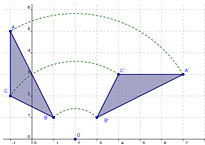
\includegraphics[scale=0.8]{rigid.png}
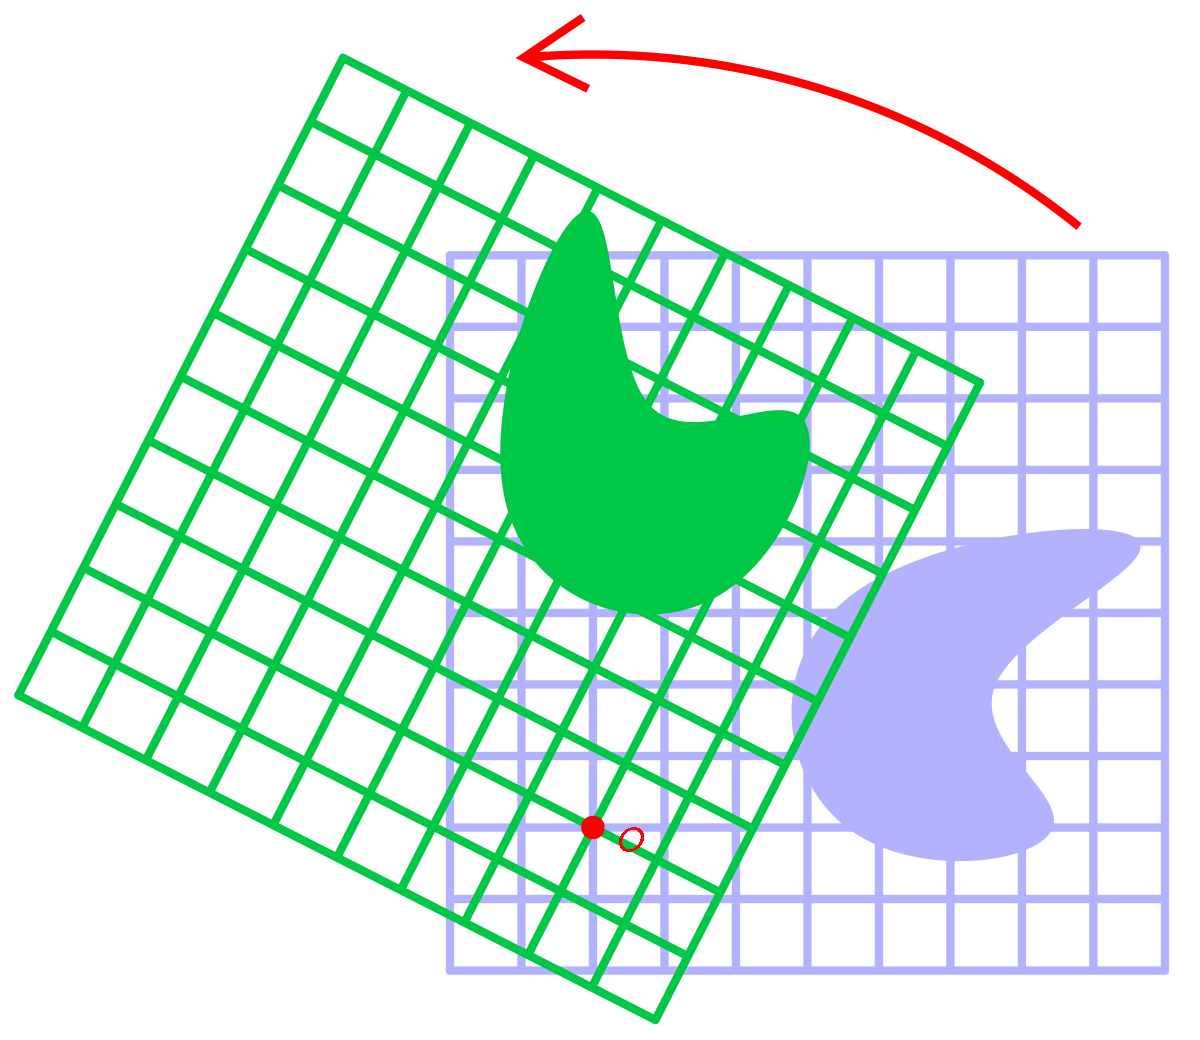
\includegraphics[scale=0.11]{fixed.png}

\end{frame}

\begin{frame}{Rotaciones en $2D$: con números complejos}

% Empecemos por las rotaciones en $\R^2$, que son más fáciles. ¿Cómo son? ¿Cómo se describen? ¿Cómo hago para [PIZARRÓN] armar una rotación (con centro en el origen) que mueva un punto $P$ a un punto $Q$ (de la misma longitud)?

% Acá los números complejos nos van a resultar muy útiles. Así que veamos qué eran.

Empecemos por las rotaciones en $2D$, usando números complejos. \bigskip



%TODO agregar imagen de conjuntos aritméticos y dejar eso en vez de esto:
\small{Nats $\rightarrow$ Enteros (tienen negativos)}

Reales $\rightarrow$ Complejos ($\rightarrow$ ¡Cuaterniones!)  \bigskip

¿Cuánto vale $\sqrt{-1}$?\ Bueno, llamémoslo $\ii$ 


¿Y qué hacemos con eso? ¿Cómo hacemos cuentas?

% Los números complejos no son nada más que un "upgrade" que led hacemos a los números que ya teníamos. En la primaria empezamos con los naturales, después nos preguntamos qué pasaba si le restábamos un número más grande a un número más chico y aparecieron los enteros, que son los que también pueden ser negativos, y para responder preguntas similares nos inventamos a los números racionales y a los reales, que son los qué conocemos más o menos bien.

% Los números complejos aparecen al responder la pregunta: "cuánto vale \sqrt{-1}"?


%PIZARRÓN: $i^2=-1$.

% Es una abstracción más, así como los números negativos son una abstracción a la que ya estamos super acostumbrados. Y...es una abstracción súper útil.

% Ahora que nos inventamos un nuevo número \textbf{i}, podemos sumarlo y multiplicarlo por otros números, obteniendo:

% PIZARRÓN: 1+i, 2+i, 3\cdot i, 2 + 3\cdot i

% Y podemos preguntarnos qué representan esos nuevos números

\end{frame}



\begin{frame}{Números complejos en el plano}

	%Y resulta que también es útil representar a los números complejos en un plano, como si tuvieran dos coordenadas. Veamos el siguiente ejemplo.
	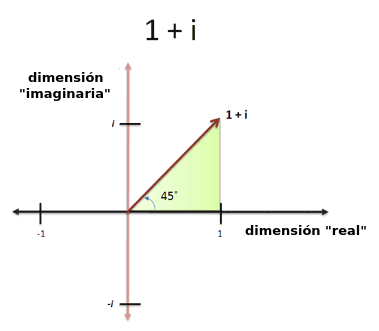
\includegraphics[scale=0.8]{1plusi.png}
	
	% Como $i^2=-1$
	% Fíjense que cuando hacemos esto, les podemos inventar dos características nuevas a los números complejos:
	
	
	\begin{itemize}
	
		% Pitágoras
		\item Longitud ('módulo'): $|1+\ii| = \sqrt{1^2 + |\ii|^2} = \sqrt{1+1} = \sqrt{2}$

		% Trigonometría, SOHCAHTOA		
		\item Ángulo: $\alpha = cos\m(\frac{CA}{HIP}) = cos\m(\frac{1}{\sqrt{2}}) = 45^\degree = \frac{\pi}{4}$
	\end{itemize}
\end{frame}

\iffalse
\begin{frame}{Conjugación}

$$x = a+b\cdot \textbf{i} \Rightarrow x^* (=\bar{x}) = a\circled{-}b\cdot \textbf{\ii}$$

% A los números complejos se los puede conjugar

% Es cambiar el signo del numerito que acompaña a \textbf{i}
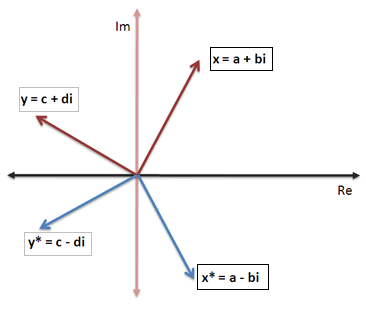
\includegraphics[scale=0.8]{conjugado.png}

%TODO ¿por qué es buena la conjugación? Porque nos re sirve para obtener inversos

\end{frame}
\fi


\begin{frame}{Forma trigonométrica}

¡Tener un número complejo es lo mismo que tener su ángulo y su módulo!
	% Copio el dibujo en el pizarrón y hago trigonometría para probar la forma trigonométrica
	
	% SOH. sen(\alpha) = \frac{CO}{HIP} \Rightarrow CO = sen(\alpha) HIP = sen(\alpha) |z|
	% CAH. cos(\alpha) = \frac{CA}{HIP} \Rightarrow CA = cos(\alpha) HIP = cos(\alpha) |z|
	
	% Entonces si tengo z = a+bi, CA = a, CO = b, y sacando factor común obtenemos...
	
	De hecho si el número es $a + b\cdot i$ entonces:
	
	$$cos(\text{ángulo}) \cdot \text{longitud} = a$$
	$$sen(\text{ángulo}) \cdot \text{longitud} = b$$
	
\iffalse
\[
	z = a + b\cdot i = \text{longitud} \cdot [\underbrace{cos(\text{ángulo})}_{a/HIP} + \ii\cdot \underbrace{sen(\text{ángulo})}_{b/HIP}]
\]

Escrito con letras:

\[
	z = a + b\cdot i = |z| \cdot [\underbrace{cos(\alpha)}_{a/HIP} + \ii\cdot \underbrace{sen(\alpha)}_{b/HIP}]
\]

\fi
\end{frame}


\begin{frame}{¿Cómo operar?}
	% Algo que pasa y que se puede demostrar con más trigonometría pero que no vamos a hacer es que cuando multiplicamos dos números complejos, lo que obtenemos es un nuevo número complejo donde los módulos se multiplican y los ángulos se suman
	
	Si $z,w$ son complejos, entonces $z \cdot w$ 'es' sumar los ángulos y multiplicar las longitudes (los 'modulos'). 
	
	
	
	¡Hagamos un ejemplo! ¿Cuánto da $(1+\ii)\cdot \i$?
	
%	Si $z = |z|\cdot [cos(\alpha) + \ii\cdot sen (\alpha)]$,\\
%	   $w = |w|\cdot [cos(\beta) + \ii\cdot sen (\beta)]$ \\
%	   entonces $z\cdot w = |z|\cdot |w|\cdot [cos(\alpha+\beta) + \ii \cdot sen(\alpha+\beta)]$
	   
	   % O sea, el módulo del nuevo número complejo es $|z||w|$, y el ángulo es $\alpha+\beta$
	   
	   % Un buen ejemplo es i^2=-1 (el módulo es 1 y el ángulo pasa de pi/2 a pi)
\end{frame}


\begin{frame}

\Huge{Muy lindo, ¿pero y con las rotaciones qué onda?}

Pensemos un poco cómo se relacionan.

% Fíjense qué bueno: si agarramos a un número complejo y lo multiplicamos por otro de módulo $1$, ¡lo estamos rotando! porque el módulo del primer complejo no cambia pero su ángulo sí.

%Hacer ejemplo en el pizarrón: 1\cdot i, (1+i) \cdot i$

\end{frame}

\begin{frame}{Ejemplo}

¿Cómo llevo el punto $(1,1)$ al punto  $(-\sqrt{2},0)$?

% PIZARRÓN dibujar
% Fíjense que necesito que los dos tengan el mismo módulo (la misma longitud), sino el problema es imposible.

% Se puede obtener el ángulo de 1+i con trigonometría pero es aburrido y además existen funciones que ya te lo hacen.

% Necesito ángulo 3/4 pi, entonces lo escribo en forma trigonométrica y listo.
\end{frame}

%TODO tal vez otra imagen sería mejor
\begin{frame}

% Los complejos de módulo 1 representan rotaciones, y fíjense que si tenés modulo 1 estás en la circunferencia de radio 1. En ese sentido el número complejo indica qué rotación es.
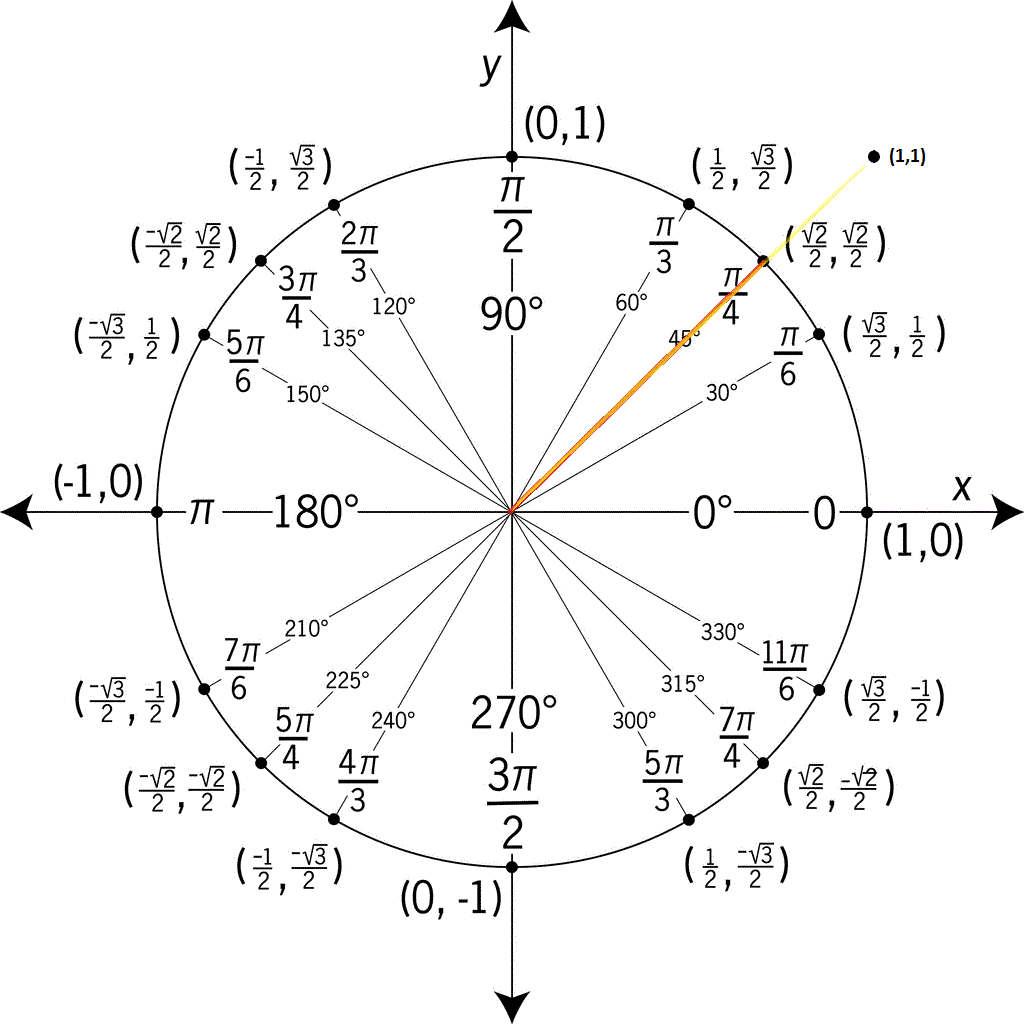
\includegraphics[scale=0.35]{unit_circle.png}

\end{frame}

\begin{frame}{¿Cómo invierto una rotación?}

%TODO Expandir
¿Será difícil? 

Si tengo $a+b\cdot \textbf{i}$ con ángulo $\alpha$ y quiero otro número complejo con ángulo $-\alpha = 2\pi - \alpha$, lo conjugo, es decir, uso $a-b\cdot\textbf{i}$

\begin{figure}
\centering
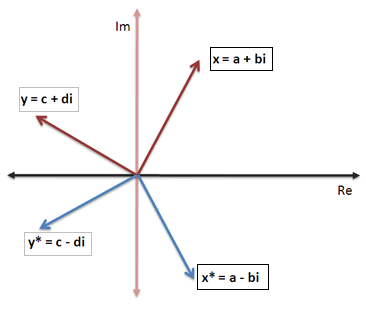
\includegraphics[scale=0.7]{conjugado.png}
\end{figure}

% Y fíjense qué copado. Cuánto da z \bar{z}? Es posta el inverso! (Si el módulo es 1)

\end{frame}



% Para el final de números complejos
\begin{frame}{Volvamos a \textbf{i}}

¿Cuál es la solución de $x^2=-1$? 

% Fíjense que esta ecuación es lo mismo que esta.

$1\cdot x^2 = -1$

% Y ahora la pregunta es: ¿qué rotación, aplicada 2 veces, lleva el 1 a -1?
% Hay que girar 2 \pi, pero haciendo dos veces la misma rotación. O sea, la rotación tiene que ser de \pi, un ángulo recto. Y qué número complejo representa un número recto? i! 



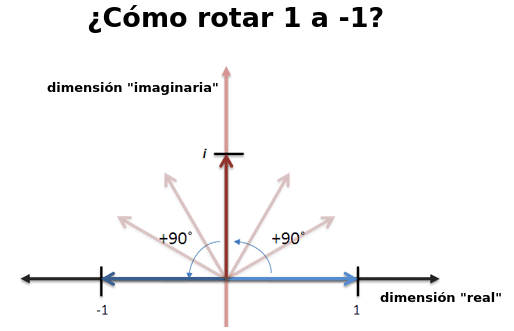
\includegraphics[scale=0.78]{rotate1m1.png}


\end{frame}


\begin{frame}{Volvamos a \textbf{i} (cont)}
	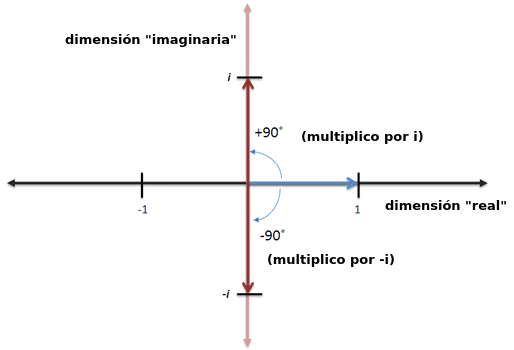
\includegraphics[scale=0.78]{rotate1m1_2.png}
	
	% Y el álgebra nos lo confirma: (-i)\cdot (-i) = (-1) \cdot i \cdot (-1) \cdot i = i \cdot i = 1$. Estamos usando que el producto es conmutativo.
\end{frame}



\iffalse

%TODO hablo de matrices? Sirve para algo?
\begin{frame}{Matrices}

% Bueno, quiero pasar ahora a otra herramienta para entender rotaciones (y más adelante, en particular, a los cuaterniones)

% Hablemos un poco de matrices.



\[
\begin{bmatrix}
    1  &  -1      \\
    0  &  2      
\end{bmatrix}
\visible<2->{\cdot
\begin{bmatrix}
    1  &  0      \\
    0  &  2      
\end{bmatrix} }
\visible<3->{=
\begin{bmatrix}
    1  &  -2      \\
    0  &  4      
\end{bmatrix} }
\]


\end{frame}

\begin{frame}{Matrices}
\[
\begin{bmatrix}
    1  &  -1      \\
    0  &  2      
\end{bmatrix}
\cdot
\begin{bmatrix}
    1  &  0      \\
    0  &  2      
\end{bmatrix}
 =
\begin{bmatrix}
    1  &  -2      \\
    0  &  4      
\end{bmatrix}
\] 

\[
\begin{bmatrix}
    0  &  -1      \\
    1  &  0      
\end{bmatrix}
\cdot
\begin{bmatrix}
      1      \\
      0      
\end{bmatrix}
=
\begin{bmatrix}
    0        \\
    1        
\end{bmatrix}
\]

\end{frame}


\begin{frame}{¿Y para qué sirven?}
Algunas propiedades:
	\begin{itemize}
		\item Representan funciones (transformaciones del espacio).
		\item Los números complejos se pueden ver como matrices
		\item Algunas matrices representan rotaciones
	\end{itemize}
\end{frame}

\begin{frame}{Las matrices como funciones (transformaciones lineales)}

$ A \leftarrow$ matriz

$ x \leftarrow$ punto ('vector') genérico de $\R^2$ (el plano) \bigskip

Puedo definir la siguiente función:

\Huge $$f(x) = A\cdot x$$

% Gracias a que cuando multiplico una matriz por un vector me da otro vector, dada una matriz me puedo definir una función.




\end{frame}


\begin{frame}{Números complejos como matrices}

Si $z=a+bi$, ¡se puede expresar como matriz! 

\[
\begin{bmatrix}
    a  &  -b      \\
    b  &  a      
\end{bmatrix}
\]

\begin{itemize}
	\item El producto de complejos se corresponde con el producto de matrices
	\item Todo anda bien
\end{itemize}
	
% Esa matriz guarda la información, con dos valores repetidos, del número complejo. O sea, el número está en la primera columna.

% Y el producto de dos complejos anda bien, veamos un ejemplo

% Que el ejemplo sea (1+i) (i)


	
\end{frame}


\begin{frame}{Algunas matrices son rotaciones}

Esto es una consecuencia de las dos slides anteriores.

Si $z =  \underbrace{cos(\alpha)}_{a} + i \underbrace{\ sen(\alpha)}_{b}$ (o sea, tiene módulo $1$), la matriz que le podemos asociar es:

\[
\begin{bmatrix}
    cos(\alpha)  &  -sen(\alpha)      \\
    sen(\alpha)  &  cos(\alpha)      
\end{bmatrix}
\] 

Este tipo de matrices representan las rotaciones en $2D$.

\begin{itemize}
	\item Forman un \textbf{grupo} conmutativo llamado $SO(2)$.
	%\item La inversa de una matriz allí es su transpuesta % Coincide con el inverso del complejo
	\item En particular, todo elemento tiene inverso. %Conviene pensar en rotaciones!
	%\item Tienen determinante $1$. % Coincide con el cuadrado del módulo del número complejo
	
\end{itemize}

% Todas estas propiedades se pueden ver tanto viéndolas como números complejos, como con matrices, o simplemente pensando en rotaciones de $\R^2$

% La idea es que elijan la manera de pensar qué más les guste pero si tienen una manera de pasar de un mundo a otro eso les puede servir para atacar un problema de varias formas distintas

% Si uno piensa un problema con el enfoque que más le conviene, pero el resultado lo tiene que dar en el otro universo, hace la traducción y listo

% Si quieren, por ejemplo, podemos tratar de entender cómo es el inverso de un número complejo de módulo 1, pensando con rotaciones.
\end{frame}

\fi


\begin{frame}{¿Qué es una rotación (en $3D$)?}

	\Huge ¿Qué es una rotación en $3D$?


% Antes de cerrar la charla quiero empezar a hablar un poco de $\R^3$ y que se note la relevancia de todo lo que discutimos en $\R^2$

	
\end{frame}

\begin{frame}{¿Qué es una rotación en $3D$? Formalismo matemático}
	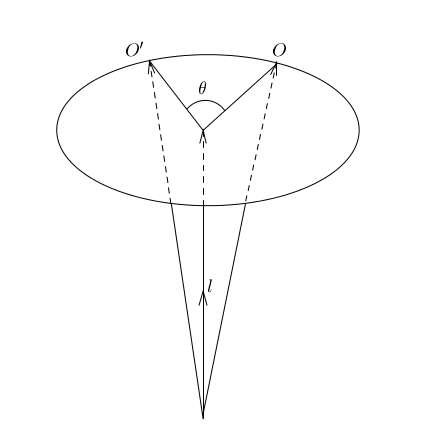
\includegraphics[scale=0.6]{rotation.png}
	
	%Una rotación de $\R^3$ está compuesta por un eje $\ell$ (que define un plano ortogonal) y un ángulo $\theta$...y ya sé lo que están pensando. Ese dibujo no se entiende.
	
\end{frame}


\begin{frame}{¿Qué es una rotación en $3D$? Un pisa papas}

%TODO El mango del pisa papas y la rejilla están a 90 grados. Y un pisapapas representa, bien en el fondo, una rotación en $\R^3$. El mango es el eje de rotación y un punto de la rejilla rota alrededor del mango con un ángulo fijo, como si fuera una rotación en $\R^2$ donde el origen está donde el mango y la rejilla se tocan.

%PIZARRÓN: hagamos el dibujito en el pizarrón
% Ojo que el pisa papas debe pasar por el origen! Sino no funciona la cosa

% ¿Cómo gira un punto que no está en la rejilla? Bueno, según una rejilla imaginaria

% Además el pisa papas puede estar inclinado de distintas maneras
	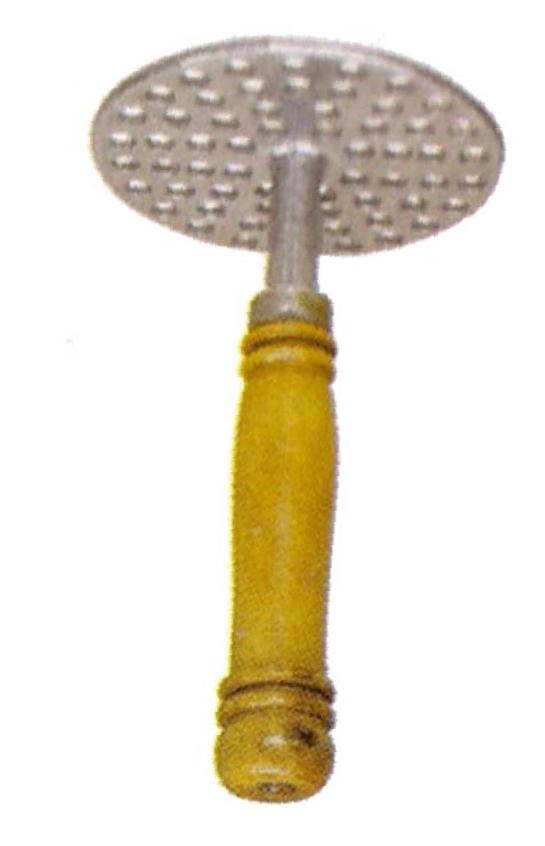
\includegraphics[scale=0.2]{pisapapas_dadovuelta.png} 
	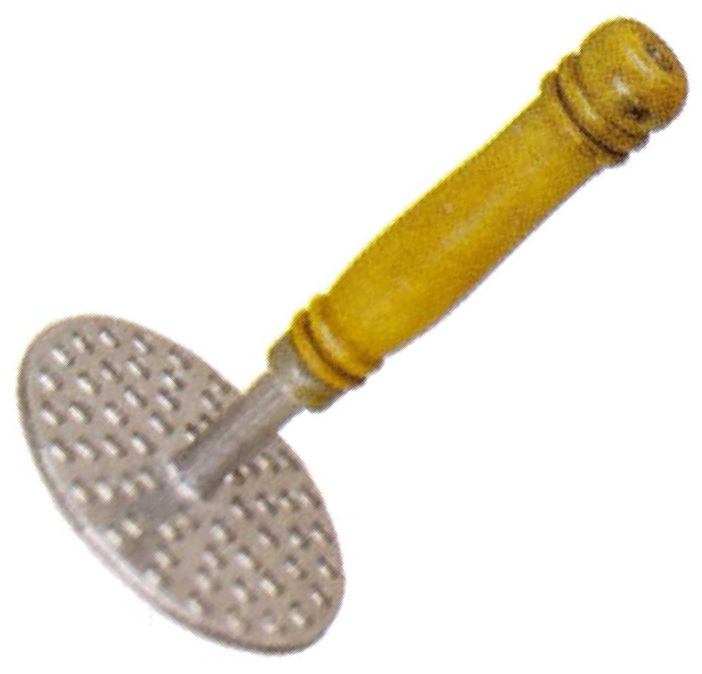
\includegraphics[scale=0.2]{pisapapas_45.png}
	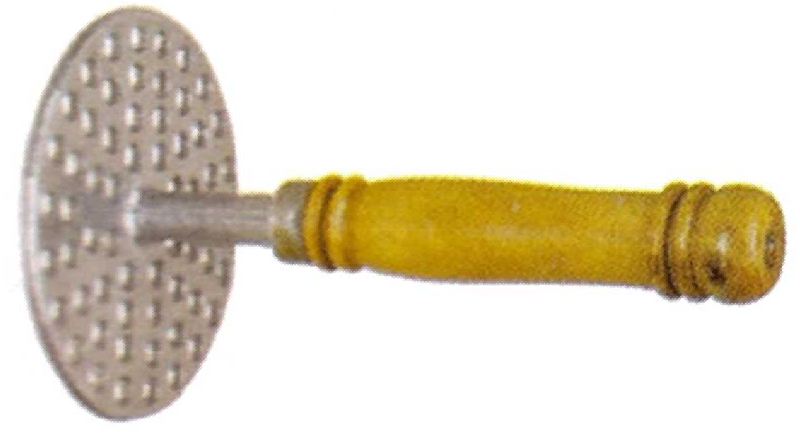
\includegraphics[scale=0.2]{pisapapas_180.png}
	
	% Fíjense que una rotación en $\R^3$ deja fija a toda una recta (el mango del pisapapas), mientras que una rotación en $\R^2$ deja fijo solo al origen. "Aumenta una dimensión" de lo que dejás quieto	
	
\end{frame}





\begin{frame}{Otro pisa papas}

	% Puede estar inclinado "en profundidad"
	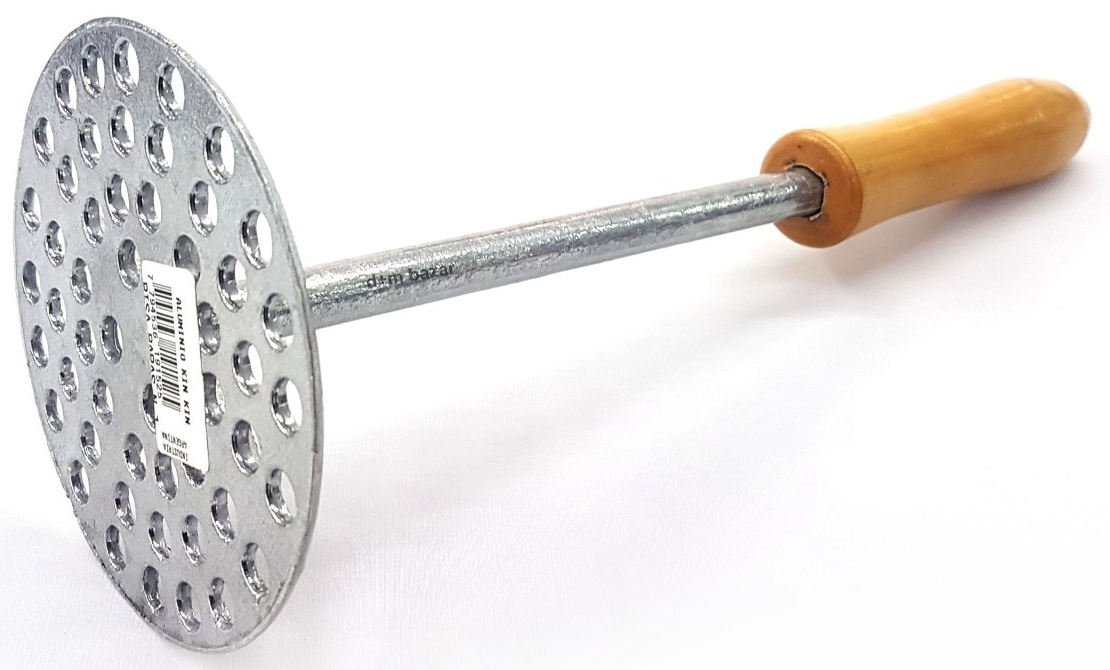
\includegraphics[scale=0.3]{pisapapas_prof.png}
	

	% Por eso son tan importantes las rotaciones en $\R^2$ para entender las que son en $\R^3$, por eso nos sirven las herramientas que aprendimos antes
	
	% Una rotación en $\R^3$ no es más que muchas rotaciones imaginarias: una por cada rejilla imaginaria - hay una por cada altura y de cada radio posible - que atraviesa de manera ortogonal al mango del pisa papas.
	
	% Entonces, ¿qué alcanza para definir una rotación en $\R^3$? En criollo pregunto.
	
	% [Pausa] ¡El mango!
\end{frame}

\begin{frame}{Por fin, cuaterniones}

	% Bueno, les presento a los cuaterniones y continuamos el jueves.
\begin{figure}  		
  	\centering
	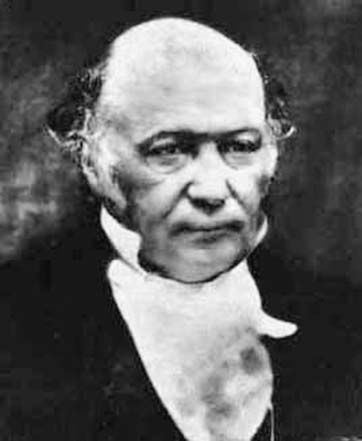
\includegraphics[scale=0.35]{hamilton_cara.png}
	\caption*{William Hamilton, el inventor de los horribles, \textit{horribles} cuaterniones.}
\end{figure} 

	% El inventor, o descubridor, si prefieren, de los cuaterniones fue un tipo que se llamaba Hamilton.
	
	% Hamilton quería generalizar el concepto de número complejo a otro objeto matemático que tuviera aplicaciones en $\R^3$
	
	% El tema es que Hamilton se imaginaba que había que agregar una sola letra imaginaria, digamos \textbf{j}. Y eso no funciona. 
Hamilton buscaba esto:
	$$a +b\cdot \textbf{i} + c \cdot \textbf{j}$$ \\
	
	($a,b,c$ son números reales) 
	
	...pero no funcionó.

\end{frame}

\begin{frame}

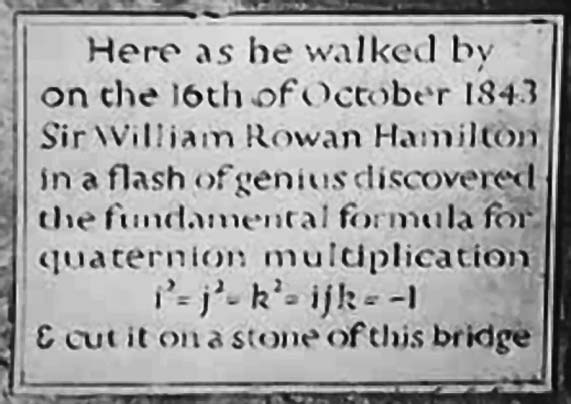
\includegraphics[scale=0.7]{hamilton.png}

\end{frame}

\begin{frame}{Cuaterniones}
Un cuaternión tiene esta pinta:
$$a +b\cdot \textbf{i} + c \cdot \textbf{j} + d \cdot \textbf{k}$$

	($a,b,c,d$ son números reales)  \\
	($\textbf{i},\textbf{j},\textbf{k}$ son números 'imaginarios')  \newline
	
	% Así como antes $i^2 = -1$ era la regla que usábamos para hacer cuenta, ahora estas van a ser las reglas
	

\center	Reglas:
	$$\textbf{i}^2 = \textbf{j}^2 = \textbf{k}^2 = \textbf{i}\cdot\textbf{j}\cdot\textbf{k} = -1$$  	
	% Hay algunas reglas más a tener en cuenta	
	$$\textbf{ij}=\textbf{k}\ \ \ \textbf{jk}=\textbf{i}\ \ \ \textbf{ki}=\textbf{j}$$
	$$\textbf{ji}=-\textbf{k}\ \ \ \textbf{kj}=-\textbf{i}\ \ \ \textbf{ik}=-\textbf{j}$$ 
	
	%O sea, i -> j -> k ->i, si multiplico dos consecutivos en orden da el otro positivo.
\end{frame}

\begin{frame}{Una representación alternativa}

Así como a un número complejo lo podíamos marcar en un plano (2 dimensiones), un cuaternión es como un vector de 4 dimensiones (no dibujable) y se puede escribir así:

$$a +b\cdot \textbf{i} + c \cdot \textbf{j} + d \cdot \textbf{k} \approx (\textbf{a},b,c,d)$$

%pero hay que tener cuidado y elegir una coordenada para que sea 'especial' ¡Fíjense que en los complejos pasaba lo mismo! La parte real era la 'especial'. Acá lo mismo.

%Se suele elegir la primera por comodidad pero tranquilamente se podría elegir otra.

\end{frame}

%TODO después de la primer charla cambiar el resumen según cómo estuvo.
\begin{frame}{Resumencito}

Los números complejos:
\begin{itemize}
	\item Se pueden marcar sumar, restar, multiplicar, dividir.
	\item Se pueden marcar en un plano.
	\item Se les puede medir la longitud y obtener el ángulo.
	\item Los de módulo $1$ representan rotaciones
	\item Para éstos, el conjugado es el inverso
	%\item Todos los complejos se pueden representar con matrices. Las matrices son el fondo funciones (transformaciones lineales)
	%\item  Algunas matrices, las que representan complejos de módulo $1$, también representan rotaciones (la función 'rotar')
\end{itemize}

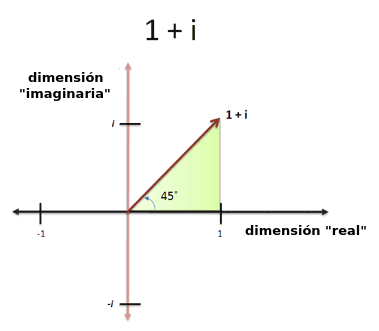
\includegraphics[scale=0.4]{1plusi.png}

\end{frame}

\begin{frame}{Resumencito II}
\begin{itemize}
	\item Las rotaciones en $3D$ son girar alrededor de un eje por un ángulo fijo (un pisapapas).
	\item Los cuaterniones nos van a servir para representarlas.
	\item Los cuaterniones son como los complejos pero con 2 letras más y por ende más reglas que solamente $i^2=-1$.%En particular, multiplicar no siempre conmuta. Tampoco las rotaciones en $3D$.
	%\item El producto de cuaterniones es asociativo. La suma de cuaterniones es conmutativa y asociativa.
	\item Así como los complejos se pueden ver como puntos en un plano ($2D$), los cuaterniones se pueden ver como puntos de 4 dimensiones (4 números).
\end{itemize}
\end{frame}

\begin{frame}{Tarea =)}
	¿Cómo se multiplican dos cuaterniones? ¡Usar las reglas que vimos! \bigskip
	
	$$(2+3\cdot \ii + 2 \cdot \jj - 4 \cdot \kk) \cdot (1-2\cdot \ii + 1 \cdot \jj + 4 \cdot \kk) = \text{???}$$
	
	
\end{frame}

\begin{frame}{¡Fin!}
\Huge ¿Preguntas?
\end{frame}



\begin{frame}{¡Cuidado!}
Ojo: El producto de cuaterniones en general no es conmutativo.

	% Fíjense que el producto NO es conmutativo en este caso.
	% Déjenme justificarles por qué el producto no es conmutativo de una manera intuitiva

	% Si los cuaterniones están relacionados con las rotaciones en $\R^3$ (lo vamos a ver la próxima clase) tiene sentido que si las rotaciones no son conmutativas entonces el producto de cuaterniones tampoco.
	
	% Las rotaciones en $\R^3$, ¿son conmutativas?
	
	% No. Y lo podemos ver con un cubo de rubik. Las rotaciones en $\R^3$ no son lo mismo que las de un cubo de rubik, pero sirven para generar intuición.
	
	% Si rotamos para abajo y para la izquierda no queda igual que primero para la izquierda y después para abajo.
	
	% Esto ya nos da una primer diferencia con $\R^2$
\end{frame}








\section{Segunda clase: cuaterniones!}


\begin{frame}{Operatoria de cuaterniones}
¿Cómo eran los cuaterniones? 

$$a + b \cdot \ii + c \cdot \jj + d \cdot \kk$$




\begin{itemize}
        \item En general no conmutan (esa propiedad se pierde)
		\item El producto de un número real y un cuaternión sí conmutan.
		\item La suma de dos cuaterniones es conmutativa
		\item La suma y el producto es asociativo		
\end{itemize} 

¿A ustedes como les aparecen cuando los usan?
	% Un cuaternión es elegir valores de a,b,c,d. Si elegimos todos cero salvo b obtenemos $i$, y si elegimos todos cero salvo $a$ obtenemos un número real
	% Y esos sí conmutan, pero no nos metamos mucho en eso.
	
	% Uno puede multiplicar usando la doble distributiva para ver cómo se llevan las letras y listo. Hagamos un ejemplo
\end{frame}

\begin{frame}{¿Y por qué no conmutan?}
    ¿Por qué en general $q_1 \cdot q_2 \neq q_2 \cdot q_1$? 
    
    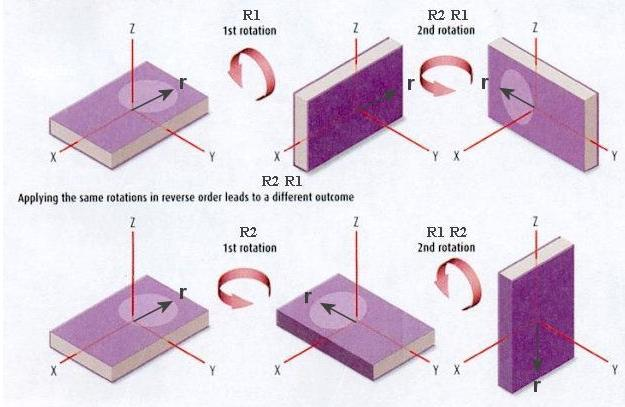
\includegraphics[scale=0.6]{dontcommute.jpg}
    
    Porque las rotaciones no conmutan.
    
\end{frame}

\begin{frame}{¡Aun hay más!}

%Hackcito porque me da paja usar align
\begin{equation}
\begin{tikzcd}
\ \ \ \ \ \ \ \ \ \ \ \ \ Sedeniones \text{\sout{(son una bosta)}}\\
Octoniones \arrow{u} \\
Cuaterniones \arrow[u, "o_1 \cdot (o_2 \cdot o_3) \neq (o_1 \cdot o_2) \cdot o_3"'] \\
Complejos  \arrow[u, "q_1 \cdot q_2 \neq q_2 \cdot q_1"', u] \\
Reales \arrow[u, "\text{todo es lindo}"'] 
\end{tikzcd}
\end{equation}


\end{frame}


%Esto hacerlo en el pizarrón
% Notación
% Les cuento de paso que a veces las cosas se abrevian así
%$q = (q_0, \textbf{q})$, donde $q=(q_0,q_1,q_2,q_3)$ y $\textbf{q}= (q_1,q_2,q_3)$

\begin{frame}{Cuaterniones como DigiEvolución de los números complejos}
\tiny{Igual a mí me gustaba más Pokemon.} \bigskip

\normalsize
%TODO llevar las reglas para operar

% DigiEvolución es algo de un dibujito, no es un término matemático, aclaro

En $2D$, si $v,z$ son números complejos, cuando los multiplico me da $v$ rotado en el ángulo de $z$

$$w = v \cdot z$$  \bigskip


En $3D$, si $v$ tiene 3 dimensiones y $q$ es un cuaternión de longitud $1$, esta cuenta me devuelve $v$ rotado 'según' el cuaternión:

$$\hat{w} = q \cdot \hat{v} \cdot q^*$$ 

\hbox{\hspace{8.5cm} 
\includegraphics[scale=0.18]{carl-sagan-dude-what.jpg}}

% Entonces hay dos cosas que queremos hacer:
% La primera es entender la fórmula
% La segunda es entender qué significa %'según' el cuaternión%
% Fíjense que aparece un cuaternión, el vector v que queremos rotar con una raya arriba, y una estrella

%PIZARRÓN escribirlo ahí para que quede

\end{frame}


\begin{frame}{Conjugación}

% Cambiemos la notación un poco, y en vez de poner a,b,c,d, pongamos q_0,q_1, q_2,q_3.
Dado $q=q_0 + q_1 \textbf{i}+ q_2 \textbf{j}+ q_3 \textbf{k}$, definimos:

$q^* = q_0 -  q_1 \textbf{i} -  q_2 \textbf{j}-  q_3\textbf{k}$ el conjugado de $q$. \bigskip


Con los complejos era parecido pero había menos letras:

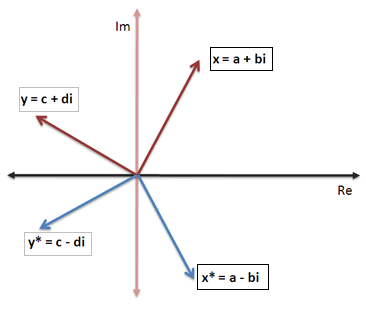
\includegraphics[scale=0.5]{conjugado.png}

\iffalse
 \bigskip



Es lo mismo que decir lo siguiente:

Si $q = (q_0, \textbf{q}
)$, entonces $\bar{q} = (q_0, - \textbf{q}
)$

% Le pongo un menos al vector de $\R^3$
\fi

\end{frame}


\begin{frame}{De paso: longitud de un cuaternión}
    
    Longitud de un número complejo $a+b\cdot \ii: \sqrt{a^2+b^2}$ \bigskip
    
    'Longitud' de un cuaternión $a+b\cdot \ii + c\cdot \jj + d\cdot \kk: \sqrt{a^2+b^2+c^2+d^2}$ 
    
    Vale que si la longitud del cuaternión es $1$, entonces el inverso multiplicativo es el conjugado.
    
    ¿Se acuerdan por qué valía con complejos?
\end{frame}

\begin{frame}{'Aumentar' $v \in \R^3$ (3 dim) a $\hat{v} \in Cuat$ }

%Bueno ya sabemos qué hace la estrella
% Ahora aparentemente si tengo un vector de $\R^3$ le puedo poner una barra arriba y eso hace que pase algo

% Lo que sucede es lo siguiente: queremos 'juntar' un vector de $\R^3$ con un cuaternión de $\R^4$, pero tienen dimensiones distintas. Así que al vector de $\R^3$ lo aumentamos. ¿Cómo? Haciendo que la parte que no tiene letra, que la gente llama "parte escalar" sea 0.

Dado $v = (v_1,v_2,v_3)$, defino $\hat{v}= 0 + v_1 \cdot \textbf{i} + v_2 \cdot \textbf{j} + v_3 \cdot \textbf{k}$ 

Lo 'aumento' para que tenga 4 dimensiones.


%Otra manera de verlo es que $ \hat{v} =(0,v)$ (y tiene $4$ dimensiones) 
%Por eso es buena esta notación
	
\end{frame}

\begin{frame}{Volvamos a la formulita}

Si $v$ es un vector de 3 dimensiones en el espacio y $q$ es un cuaternión de longitud $1$, esta cuenta me devuelve $v$ rotado 'según' el cuaternión:

$$\hat{w} = q \cdot \hat{v} \cdot q^*$$ 

Pasos:

\begin{itemize}
	\item 'Aumento' al vector $v$
	\item Lo multiplico por $q$
	\item Lo multiplico por $q^*$, que es el conjugado de $q$
	\item Eso rota $v$, pero, el resultado queda 'aumentado' (o sea, la parte escalar, que no acompaña a ninguna letra, es $0$)
	
	
	% Vamos a hacer un ejemplo pero primero entendamos QUÉ rotación representa ese cuaternión
\end{itemize}
\end{frame}


\begin{frame}{Multiplicar los cuaterniones es como componer las rotaciones}

    ¿Pero en qué orden? 
    
    Si tengo:
    
    $$\hat{v_2} = p \cdot \hat{v_1} \cdot p^*$$
    
    y luego hago:
    
    $$\hat{v_3} = q \cdot \hat{v_2} \cdot q^*$$ 
    
    Esto es lo mismo que:
    
    $$\hat{v_3} = qp \cdot \hat{v_2} \cdot (qp)^*$$
    
\end{frame}
\begin{frame}

    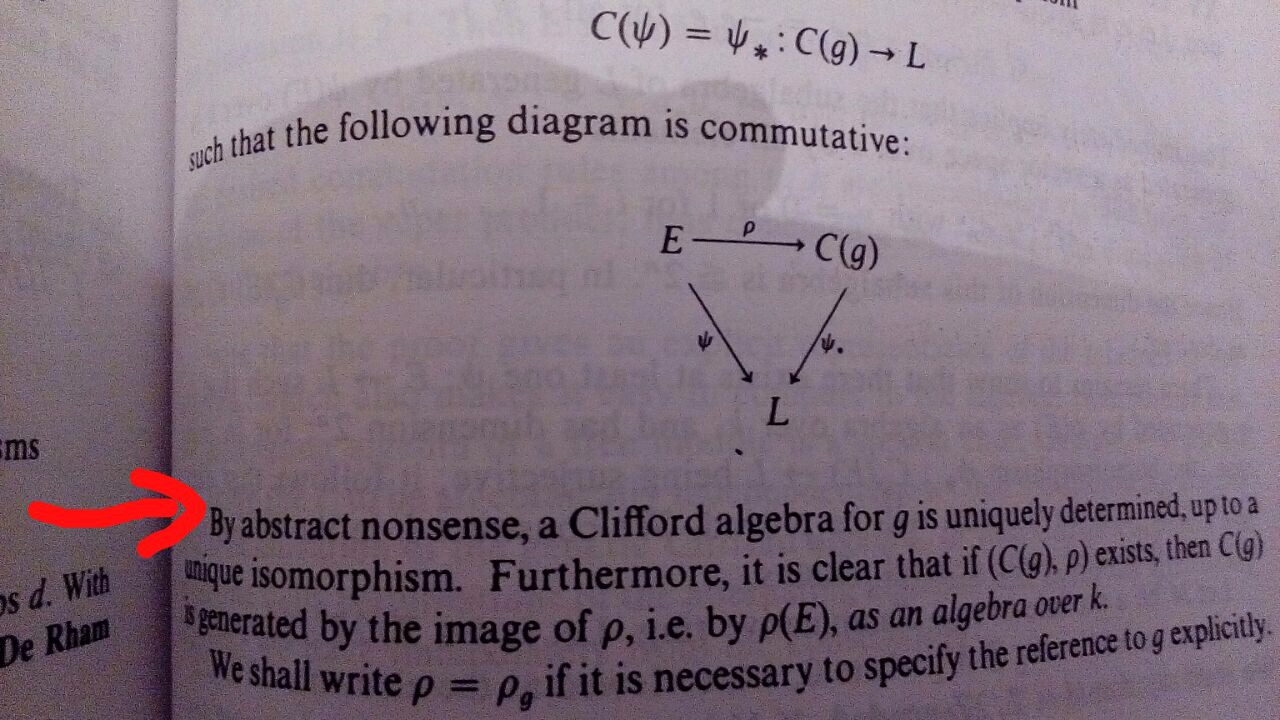
\includegraphics[scale=0.4]{nonsense.JPG}
    
\end{frame}




\begin{frame}{Slide optativa: ¿por qué necesitamos dos números más que en $2D$?}

\large Hay dos cuentas que muestran por qué no anda agregar sólo \textbf{\ii} y \textbf{\jj}:

\normalsize

\begin{itemize}
    \item Porque necesitamos 4 letras para describir a todas las rotaciones en $3D$. 
    \item Si usáramos sólo $\ii$ y $\jj$ el álgebra se rompería. (Suponés que $\ii\jj=a+b\ii+c\jj$, multiplicás a izquierda por $\ii$ y llegás a algo imposible)
\end{itemize}

\iffalse Pero supongamos que anda esto de usar 3 variables  Las podríamos representar con un vector $(x,y,z)$ o con "números" de la forma $a+b\ii+c\jj$. \\

Hamilton quería que $i^2=j^2=-1$ para generalizar a los números complejos.


¿Qué pasa cuando multiplicamos $\ii$ por $\jj$? Da...algo. Digamos que deben existir $a,b,c\in\R$ tal que $\ii\jj=a+b\ii+c\jj$. Pero multiplicando a cada lado por $\ii$ obtenemos $-j = a\ii-b+c\ii\jj$. Pero...ya sabemos cuánto vale $\ii\jj$. Reemplazando, obtenemos lo siguiente:

$-\jj=a\ii-b+c(a+b\ii+c\jj)$, o sea, $0=(ac-b)+\ii(a+bc)+\jj(c^2+1)$. Y esto implica que $c^2+1 = 0$, lo cuál no puede ser.
\fi
\end{frame}

\begin{frame}{Los cuaterniones como rotaciones (con ejemplo)}
%Si $u\in\R^3, r\in\R$, entonces $q=r(cos\theta+u\ sin\theta)$ es una rotación de ángulo $2\theta$ a través de $u$.

%¿Qué significa esto?

Si tenemos el eje (el mango del pisapapas) y el ángulo con que queremos rotar, es inmediato definirse el cuaternión que describe \textit{esa rotación}: 

Si $N= (n_x,n_y,n_z)$ es un punto (vector) de longitud $1$ (el mango del pisapapas) y $\theta$ es un ángulo, entonces: 
$$q = cos(\theta/2) + sen(\theta/2)\ n_x\ \textbf{i} + sen(\theta/2)\ n_y\ \textbf{j} + sen(\theta/2)\ n_z\ \textbf{k}$$
% Es como la forma trigonométrica de los complejos
% que tenía el ángulo bien a la vista.

representa una rotación en los planos perpendiculares a $\hat{n}$ con ese ángulo. 

(¿con complejos era parecido?)

%TODO regla de la mano derecha

%TODO escribir ANTES que los cuaterniones tienen que tener módulo 1?

 Observaciones: 

\begin{itemize}
	\item Si uso $q$ ó $-q$ obtengo la misma rotación. Pero, salvo esto, por cada rotación del espacio hay un sólo cuaternión que la representa.
	\item Con $q=1 + 0\ \textbf{i} + 0\ \textbf{j} + 0\ \textbf{k}$ obtengo la rotación 'no hacer nada'. %(ver en el pizarrón)
\end{itemize}

%Una manera más compacta de escribir la fórmula de arriba es la siguiente:

$$q(\theta, \hat{n}) = (cos(\theta/2), \hat{n}\ sen(\theta/2))$$

% PIZARRÓN: escribirla para que quede y la pueda usar para explicar por qué se dobla el ángulo

%Hacer ejemplo: pasar v=(1,0,1) a (0,1,1) usando el eje (0,0,1), que tiene módulo 1, y ángulo pi/2.

% Por trigonometría, sen(pi/4)=cos(pi/4) = \frac{sqrt[2]{2}}{2}

\end{frame}

\begin{frame}{¿Por qué multiplicamos el ángulo por $2$?}

Dos razones:

\begin{itemize}
    \item como estamos multiplicando dos veces por el cuaternión necesitamos que cada uno 'tenga' la mitad del ángulo de rotación.
    \item Si \textbf{no} multiplicáramos el ángulo por dos, tendríamos el siguiente problema (dibujito)
\end{itemize}

%TODO acordarse de dibujar la esfera!

%PIZARRÓN: Dibujar circunferencia para 1 axis, con pi/2 (ángulo recto) que representa una rotacion en pi

%PIZARRÓN: Dibujar circunferencia para 2 axis, con pi/2 en x que representa una rotación en pi, e ídem para y

% Bueno, cuando podemos rotar en 3 ejes distintos necesitamos una esfera de 4 dimensiones y no la vamos a poder dibujar, así que analicemos el caso en el que solo nos interesa rotar un punto de $\R^3$ pero alrededor del eje x o el eje y (o los nombres que quieran)

% (En la esfera de 4 dimensiones la idea es la misma pero no lo podríamos hacer de manera gráfica)

% Si los ángulos no se doblaran, tendríamos que rotar \pi grados alrededor de un eje daría lo mismo que \pi grados alrededor del otro! Pero esto no es cierto

%TODO Es cierto que un cuaternión que está en la esfera pero rotado en x representa una rotación alrededor del eje x?

\end{frame}

\iffalse
\begin{frame}{Los cuaterniones se pueden llevar a matrices}

Dado un cuaternión $q=q_0 + q_1 \textbf{i} + q_2 \textbf{j} + q_3 \textbf{k}$, la rotación que representa se puede dar con: 

\[
A = \begin{bmatrix}
    (q_0^2+q_1^2-q_2^2-q_3^2)  &  2(q_1 q_2 - q_0 q_3) & 2(q_1 q_3 + q_0 q_2)      \\
    2(q_1 q_2 + q_0 q_3) & (q_0^2 - q_1^2 + q_2^2 - q_3^2) & 2(q_2 q_3 - q_0 q_1) \\
    2(q_1 q_3 - q_0 q_2) & 2(q_2 q_3 + q_0 q_1) & (q_0^2 - q_1^2 - q_2^2 + q_3^2)
\end{bmatrix}
\]

%TODO cambiar a a,b,c,d?


$$v \mapsto A\cdot v$$
%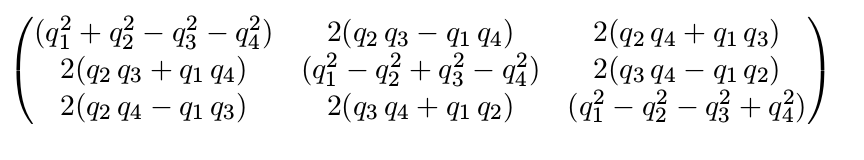
\includegraphics[scale=0.5]{quaternion_matrix.png}
\end{frame}

\fi

\iffalse
\begin{frame}{Frame Title}
    Hablar de exponenciación de raeles y complejos
    Con QuaternionReport1 puedo definir el Slerp como una exponenciación.
    
    Visualizing Quaternions pagina 102
    
    Usamos el producto para mantener módulo $1$.
\end{frame}



\begin{frame}{SLERP (interpolación a velocidad constante)}

\end{frame}

\begin{frame}{SLERP (interpolación a velocidad constante)}

%TODO q y -q representan la misma rotación
\Huge{TODO decir que el slerp puede ir por el camino largo o corto} %http://caig.cs.nctu.edu.tw/course/CA/Lecture/slerp.pdf
%Justamente la diferencia entre q y -q se da en el SLERP :D


¿Qué significa esto? Creo que es elegir el segundo cuaternión con el signo para que el producto de positivo, ver link. Eso hace que el camino sea el más corto.
% long way y short way
% https://en.wikipedia.org/wiki/Slerp#Quaternion_Slerp
%Ah! es que la rotación en el plano que te queda te la vuelta corta o la vuelta larga.

%Los cuaterniones son puntos de $R^4$ de módulo 1: están en una especie de esfera de 4 dimensiones que no nos podemos imaginar.

¿Cómo hacemos si queremos rotar un punto de $v$ a $qvq\m$ pero de manera 'continua', a velocidad constante? O, más difícil, si tenemos un vector $v$ ya rotado, o sea, tenemos $p v p\m$ y lo queremos rotar a $q v q\m$? Esto generaliza el caso anterior tomando $p = 1$ 

¡Movemos \textit{los cuaterniones}!

% Tienen que re tener en la cabeza que tienen módulo 1

% Creo que es así: lo que uno hace es mover el cuaternión por la esfera. % Esfera de cuatro dimensiones

%Imaginémonos por un segundo que no nos queremos mover por una esfera sino por 'numeritos' (ojo que no son puntos en esta simplificación). Allá lejos y hace tiempo, en la secundaria, aprendimos a hacer esto. Es una función lineal que pasa por dos puntos.




\end{frame}

\fi


\begin{frame}{SLERP: interpolación a velocidad constante}

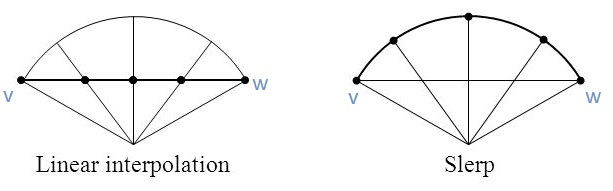
\includegraphics[scale=0.66]{Slerp2.jpg} \bigskip

¿Cómo hacemos si queremos rotar un punto $v$ a otro punto llamado $w$ a velocidad constante? 

Necesariamente $w$ debe ser $v$ rotado, por un quaternión $q$. O sea, $\hat{w}=q\hat{v}q\m$. 

\end{frame}

\begin{frame}{SLERP: interpolación a velocidad constante (cont)}

Resolvamos un problema más 'genérico' (es más fácil así):

Tenemos $p\hat{v}p\m$ y lo queremos mover a $q\hat{v}q\m$.

(Si tomamos $p=1$ recuperamos el problema original) 

¿Cómo hacemos? 

¡La idea va a ser olvidarnos del vector $v$ y mover los cuaterniones!

\end{frame}

\begin{frame}{Primero con numeritos}

Queremos mover $p$ a $q$. Finjamos primero que no son cuaterniones, sino numeritos reales. 


%PIZARRÓN: función lineal con eje x igual al tiempo y eje y igual 

% Es un sistema de ecuaciones lineales, con dos ecuaciones y dos incógnitas, sarasa

$$f(t) = (1-t) \cdot p + t\cdot q$$

$f'(t) = - p + q$: se mueve a velocidad constante.  \bigskip


Nota: la misma formulita en 3D anda bien.

% En 0 da p, en 1 da q
%PIZARRÓN: la fórmula

\end{frame}

\begin{frame}{Ahora en la circunferencia}

% PIZARRÓN dibujarla

\begin{figure}  		
  	\centering
	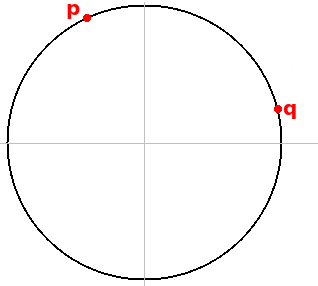
\includegraphics[scale=0.5]{slerpR2_p.png}
\end{figure}

Quiero una función $f(t)$ tal que $f(0) = p, f(1) = q$, y además $f'$ constante (para tener velocidad constante)

$f(t) = (1-t) \cdot p + t\cdot q$ anda en el sentido de que también se mueve a velocidad constante.

Pero...no se queda en la circunferencia.

%TODO dibujo


\end{frame}


\begin{frame}{Ahora en la circunferencia (II)} %TODO titulo
$$f(t) = (1-t)\cdot p + t\cdot q$$

\begin{figure}  		
  	\centering
	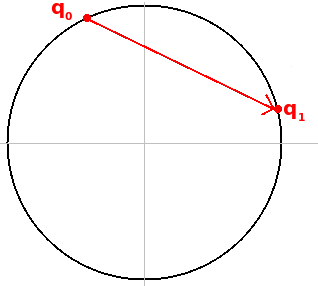
\includegraphics[scale=0.5]{slerpR2_2_p.png}
\end{figure} 

¿Cómo hacemos para que vaya por la circunferencia? 

\end{frame}

\begin{frame}{Ahora en la circunferencia(III)}

\begin{itemize}
	\item Los puntos de la circunferencia son los que tienen módulo $1$
	\item Si $(x,y) \in \R^2$, entonces $\frac{(x,y)}{||(x,y)||}$ tiene módulo 1, y está en la circunferencia.
\end{itemize}

$$f(t) = \frac{(1-t) \cdot p + t\cdot q}{||(1-t)\cdot p+ t\cdot q||}$$

\begin{figure}
  	\centering
	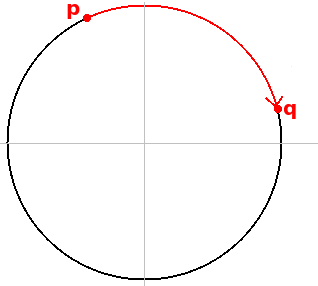
\includegraphics[scale=0.44]{slerpR2_3_p.png}
\end{figure}

Pero...no va a velocidad constante. Hay que arreglar un poco las cosas.

\end{frame}

\begin{frame}{¿Y con cuaterniones?}

%TODO agregar negrita para q_2 y q_2


$$(1-t) \cdot p + t \cdot q$$

Una vez arreglada la función para que la velocidad quede igual a $1$, sirve para puntos en el plano, y también cuaterniones:

$$Slerp(p,q,t) = \frac{sen(\textbf{(1-t)}\theta)}{sen(\theta)} p + \frac{sen(\textbf{t}\theta)}{sen(\theta)} q$$ 

¡Fíjense la simetría que tiene!

%PIZARRÓN: mancha fea SOBRE módulo de mancha fea.

($\theta$ se obtiene a partir de $p$ y $q$, es 'el ángulo' entre ellos)

%TODO SLERP es y para que se usa

\end{frame}


\begin{frame}{Volvamos a interpolación de numeritos}

$$f(t) = (1-t) \cdot p + t \cdot q$$

Es lo mismo que:

$$f(t) = p-t\cdot p + t\cdot q = p + (-p+q) \cdot t$$ 

Esa idea se puede trasladar a cuaterniones, miremos cómo:

$$f(t)= p (p^*q)^t$$ 

donde $\textit{elevar a la $t$}$ es algo parecido a la exponenciación que todos conocemos de los números reales. 

Y como al multiplicar dos cuaterniones se multiplican los módulos, todo anda bien.

\end{frame}

\begin{frame}{Resumencito III}

\begin{itemize}
    \item Los cuaterniones son un upgrade de los complejos.
    \item Tienen más letras y eso les hace perder la conmutatividad.
    \item Necesitamos agregar dos letras más porque las necesitamos para 'describir' el $\textbf{eje}$ de rotación y el \textbf{ángulo}
    \item Rotar con cuaterniones es como complejos pero un poco más feo, multiplicando a izquierda y a derecha por $q$ y haciendo un par más de cosas
    \item Como multiplicamos dos veces por $q$, si queremos rotar en un ángulo $\theta$, al cuaternión lo inventamos con $\theta/2$.
    \item Así como a los complejos se los puede describir con la longitud y el ángulo, a los cuaterniones se los puede describir con 'la normal' (o sea, 'el mango'), y el ángulo. Y de esa manera la rotación queda bien a la vista.
    \item Para rotar puntos a velocidad consante, rotamos los cuaterniones correspondientes a velocidad constante.
    
\end{itemize}
    
\end{frame}

\begin{frame}{Fin}

% TODO imagen graciosa de rotaciones
% Girando, girando hacia la libertad

\includegraphics[scale=0.4]{chiste2.jpg} \\
\Huge{¿Preguntas?}
\end{frame}



\iffalse


\begin{frame}{Cuaterniones como rotaciones}
¿Por qué necesitamos 3 letritas y no basta con 2? ¿Hago la cuenta?

Unir esto con "dimensiones": necesito $n$ grados de libertad porque sarasa.

OJO que tienen que ser unitarios los cuaterniones, creo.

\end{frame}

\begin{frame}{Regla de la mano derecha}
\end{frame}

\begin{frame}
	Cuaterniones: 'la suma de un escalar y un vector'
	El producto de cuaterniones se define con la doble distributiva y las reglas de la slide que vimos hace un rato.
	¿Cómo actúa un cuaternión sobre un vector de $\R^3$? Un vector de $\R^3$ se puede ver simplemente como un cuaternión tal que su parte real es $0$. Me parece que vamos a terminar multiplicándolos y listo.

	
\end{frame}

\begin{frame}{Resumencito}

\end{frame}

\begin{frame}

\end{frame}

\begin{frame}{¿Preguntas?}

\end{frame}




%---------------------------- "Borrador de charla" ----------------------------%

\begin{frame}{Resumen}
	La idea de la charla es hablar de cuaterniones. Los cuaterniones son una especie de números complejos en $\R^4$ (con $i,j,k$ en vez de sólo $i$), así que va a convenir hablar primero de números complejos. Además, los números complejos representan rotaciones en $\R^2$, así que va a convenir empezar por ahí.


\end{frame}


\begin{frame}{Rotaciones en $\mathbb{R}^2$}
 Números complejos al ataque.
 
 Regla: los módulos se multiplican y los ángulos se suman.
 
 NO hablar de forma trigonométrica (¿se llamaba así o me estoy confundiendo?) salvo que me sobre tiempo.
 
 Estaría bueno hacer algunas cuentitas, para entender eso de los ángulos, en realidad.
 
 Observar que para rotaciones vamos a necesitar módulo $1$.
\end{frame}

\begin{frame}
	¿Qué es un número complejo? ¿Cómo se representan en el plano complejo? ¿Qué es su ángulo? ¿Y su módulo?

	Cuando dos números complejos se multiplican, se suman los ángulos y se multiplican los módulos. Ejemplo: $(3+4i) \cdot (1+i) = 3-4 + (4+3)i = -1 +7i$; los módulos eran $5,\sqrt{2}$ y $\sqrt{50}$. Los ángulos salen de un dibujito, fue. Puedo poner $(1+i)$ rotado, pegado, al lado de $3+4i$ para que se note.
	
	Fíjense que con esta operación el $0$ sigue el elemento absorbente, el $1$ sigue siendo el neutro, todo bien. (Decirlo en criollo). Y si multiplicamos dos números reales es lo mismo de siempre, etc.	
	
	
	Las rotaciones con centro en el origen (se dice así) entonces, pueden ser dadas por números complejos de módulo $1$. ¿Cómo conocemos el ángulo de un número complejo? Con trigonometría. Senos y cosenos. Y obtenemos $z=a+bi = |z| (cos(\theta) + i sen(\theta)$.

Y fíjense qué lindo, la inversa de una rotación es simplemente usar $2\pi-\theta$, y la composición de dos rotaciones es multiplicar los números complejos correspondientes, etc.
\end{frame}

\begin{frame}
	%TODO resaltar con distintos colores
	
	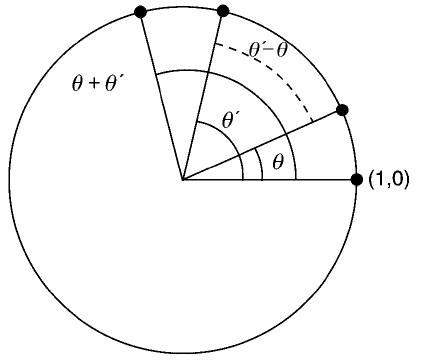
\includegraphics[scale=1]{R2.png}
\end{frame}

\begin{frame}
	No sé si hacer un ejemplo de a partir de dos vectores conseguir la rotación correspondiente. Creo que sí.
\end{frame}

\begin{frame}
	Preguntas para pensar:
	
	\begin{itemize}
		\item ¿Qué rotación me lleva el $1$ al $i$? Pensar qué ángulo necesito
	\end{itemize}
\end{frame}


\begin{frame}{Matrices}
	Ahora bien, todo esto tiene que ver con matrices.
	
	Recordar producto de matrices, y escribir matrices en latex :-)

Si $z=a+bi$, funciona tratar a los complejos como si fueran matrices. Así:

$$a, -b$$
$$b, a$$

Pero haciéndolo con ángulos y determinante $1$, queda:

$$cos(\theta), -sen(\theta)$$
$$sen(\theta), cos(\theta)$$

donde la matriz es re especial: $A^2 = Id, det(A)=1$.



\end{frame}


\begin{frame}{¿Qué es una rotación (en $\R^3$)?}
	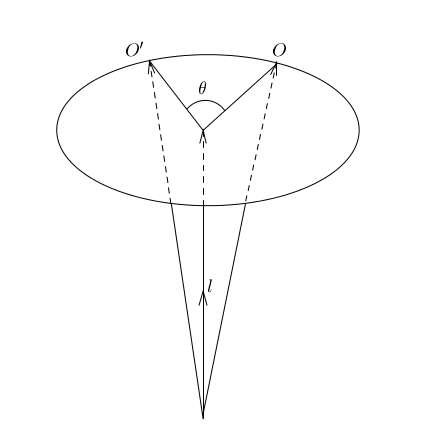
\includegraphics[scale=0.6]{rotation.png}
	
	Una rotación está compuesta por un eje $\ell$ (que define un plano ortogonal) y un ángulo $\theta$.
	
	Para cada plano ortogonal, lo que tenemos es una rotación en $\R^2$! Lo que no estoy seguro es de dónde sale el ángulo de rotación. Será el del cuaternión? Será bien visible?
\end{frame}

\begin{frame}{Ángulos de Euler}
	Los ángulos de Euler no sé lo que son exactamente, pero se usan rotaciones a través de los 3 ejes (y eso basta para representar cualquier rotación)	
	%TODO ver cómo es el teorema!
	
	Lo malo es que no es única la descomposición. Hagamos algún ejemplo.
	%TODO hacer ejemplo de dos maneras distintas.
	
	¡Además importa el orden! En ese sentido las rotaciones en $R^3$ no son conmutativas (mientras que en $R^2$ sí). Llevar cubo rubik.
\end{frame}

\begin{frame}{Ángulos de Euler (cont)}
	Los ángulos de Euler se pueden representar con matrices. ¿Recuerdan cómo operar con matrices? Hagamos algún ejemplo.
	
	Entonces, una rotación usando ángulos de Euler se pueden hacer multiplicando con 3 matrices distintas. No sé si recuerdan pero el producto de matrices en general no es conmutativo. En el apéndice $B$ de QuaternionReport está la rotación en cada eje, y se pueden usar de ejemplo.
\end{frame}

\begin{frame}{Cuaterniones}
	Los cuaterniones fueron desarrollados por Hamilton en un intento de generalizar $\C$ para que sea aplicable a $\R^3$. El tipo pensaba que bastar una coordenada imaginaria más, llamémosla $j$. Long story short, eso no se puede. Pero (literalmente) un día estaba caminando y se le ocurrió probar con 4 dimensiones y se imaginó las reglas que tenía que usar y las escribió en un puente y sarasa.
\end{frame}

\begin{frame}
	Lo que escribió en el puente fue esto:
	
	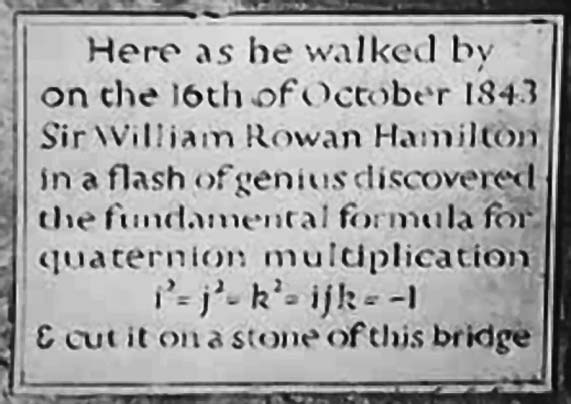
\includegraphics[scale=0.5]{hamilton.png}
	%$$i^2 = j^2 = k^2 = ijk = −1$$
	
	Y yo les podría decir que los cuaterniones son super parecidos a los complejos pero con dos letritas más y reglas adicionales....y lo son, pero hay que meterse de a poco en como \textit{operar} con ellos.
	
	La formulita escribirla en un papel.
\end{frame}


\begin{frame}{No sé si contar esto: por qué no anda con 3 dimensiones}

La idea es que un cuaternión represente una rotación. Y uno se puede preguntar por qué, dado que dos variables (números complejos) sirven para representar rotaciones en $\R^2$, no se usan 3 variables para rotaciones en $\R^3$.


%TODO arreglar las comillas
Pero supongamos que anda esto de usar 3 variables  Las podríamos representar con un vector $(x,y,z)$ o con "números" de la forma $a+b\ii+c\jj$. \\

Hamilton quería que $i^2=j^2=-1$ para generalizar a los números complejos.


¿Qué pasa cuando multiplicamos $\ii$ por $\jj$? Da...algo. Digamos que deben existir $a,b,c\in\R$ tal que $\ii\jj=a+b\ii+c\jj$. Pero multiplicando a cada lado por $\ii$ obtenemos $-j = a\ii-b+c\ii\jj$. Pero...ya sabemos cuánto vale $\ii\jj$. Reemplazando, obtenemos lo siguiente:

$-\jj=a\ii-b+c(a+b\ii+c\jj)$, o sea, $0=(ac-b)+\ii(a+bc)+\jj(c^2+1)$. Y esto implica que $c^2+1 = 0$, lo cuál no puede ser.


\end{frame}

\begin{frame}
	En algún momento quiero mencionar que vamos a trabajar con unit-length quaternions, o sea, en una esfera en $\R^4$, y que por lo tanto tienen solo 3 grados de libertad.
	
	¿Es verdad que necesito 4 numeritos para dar el eje y el ángulo? Para mí sí, total el eje lo puedo dividir por cualquier número para normalizar el cuaternión...igual no estoy tan seguro. Pero si esto es verdad tengo que decidir entre si contarlo, o lo de los 3 grados de libertad, porque ambas cosas confunden.
\end{frame}

\begin{frame}{Cuaterniones (cont)}
	Cuando hable de ellos tratarlos como ángulo + vector de $\R^3$. Y notar que eso se corresponde bien con una rotación!
\end{frame}


\begin{frame}{Gimbal lock}
Mencionar el incidente de Apollo, página 23 de Visualizing Quaternions.djvu. Incluir imágenes


\end{frame}

\begin{frame}
Podría hablar acá de diferencias entre rotaciones, ángulos de Euler y cuaterniones.

Ver página 30 del quaternion report. Igual no me cabe mucho la idea.

Idea: hacer una tabla, y poner que la gran desventaja de los cuaterniones es que son "complicados", y actualizar la slide marcando en rojo y diciendo "bueno, tratemos de eliminar esto"
\end{frame}

\fi

\end{document}
